%!TEX program = xelatex
%!TEX root = ./thesis.tex

\section{Experiment on Flat Reinforcement Learning Solutions to Multi-modality Tasks}
\subsection{Conventional Flat reinforcement Learning Methods}\label{sec_multi_modal_flat}
Contemporary end-to-end flat reinforcement learning methods may not be good at solving tasks with multi-modal state space. 
%We suggest that one of the m reason is the image features are much harder to learn than the state. The agent would tend to stuck at a local minimum when it has already learned the state features well, but has not been able to extract any useful information from the image. However, when the agent has finally learned the image features, the policy already converge to a relatively low-entropy distribution, and contemporary reinforcement learning methods cannot perform exploration again at this phase.

Take the task movecont as an example. In this task, a goal direction as sampled uniformly at random from the continuous range of angles: $[0,2\pi)$, at the beginning of each episode. The agent can only obtain the information about the target direction from the image, where there is a sphere object at the corresponding position. It is easy for the agent to learn to balance itself and stay at a stable pose based on the current motion sensor readings, in order to reduce the control cost and contact cost, as well as preventing the game over condition. However, the agent needs to extract the location of the sphere object in the image and move toward the object to solve the task. Learning the image features takes much more data than learning from the motion sensor readings, and the agent may fail to learn anything meaningful from the image while focusing on the motion sensor features. Even if the agent finally manages to extract image features, the policy might have already at a low-entropy distribution, and would not be able to make the necessary explorations for the optimal solution. Therefore, an efficient exploration technique is needed for this kind of tasks with multi-modal state space.

We would first like to examine the effectiveness of the conventional entropy regularization method for encouraging exploration of reinforcement learning agents with continuous action space. We use a multi-modal ACKTR agent. The agent uses separate networks for actor and critic function approximation with the same architecture. The image input gets feed into 3 convolutional layers with filter size 3 by 3 and stride 2, with 16, 8, 4 filters respectively. The output features of the convolutional network are passed to a fully-connected layer of 16 units. The output 16-unit fully connected layer is then concatenated with the motion sensor inputs. Finally, the concatenated feature layer is feed into 2 fully connected layers with 64 units and output the mean parameter of the policy. 

The experiment result on the entropy regularization technique is shown in Figure~\ref{rec_ent_reg}. The agents are trained using the ACKTR algorithm minibatch size 2560 and KL-divergence constraint 0.0003. The samples are produced by 32 parallel agents.The result shows that the agent easily fails to learn the reinforcement learning task when the weight of entropy term is a little bit too large. 

The average Standard Deviation of the policy distribution during training is visualized in Figure~\ref{rec_std_ent_reg}. The figure shows that the entropy regularization term might too much bias on the agent to perform exploration instead of improving its performance.
\begin{figure}[!htbp]
	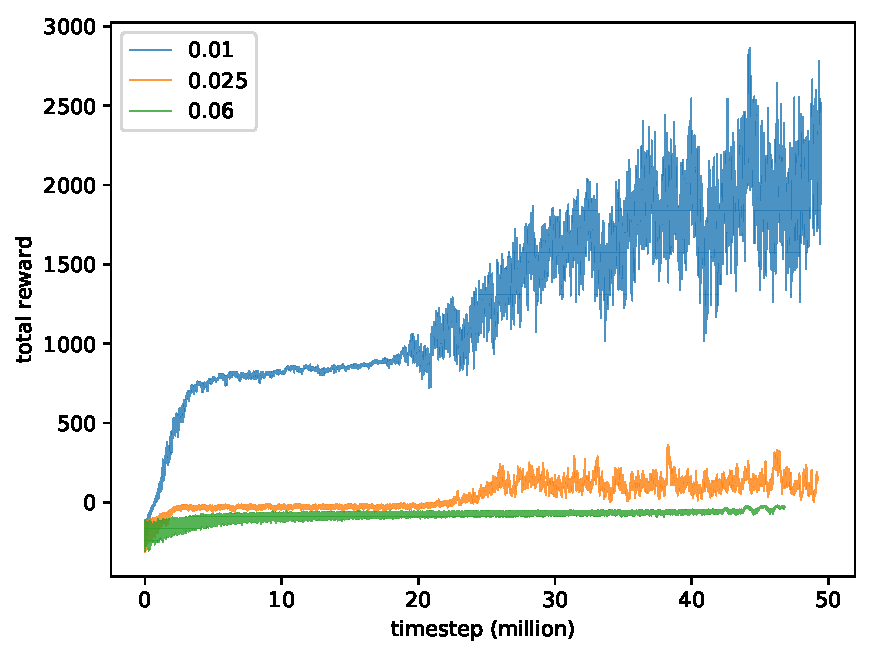
\includegraphics[width=\textwidth]{images/rec_180609_ent_reg.pdf}
	\centering
	\caption{Performance of agents with different weight on entropy regularization term, the horizontal axis is the number of million timesteps and the vertical axis is the total episode reward averaged over the last 32 episodes}\label{rec_ent_reg}
\end{figure}

\begin{figure}[!htbp]
	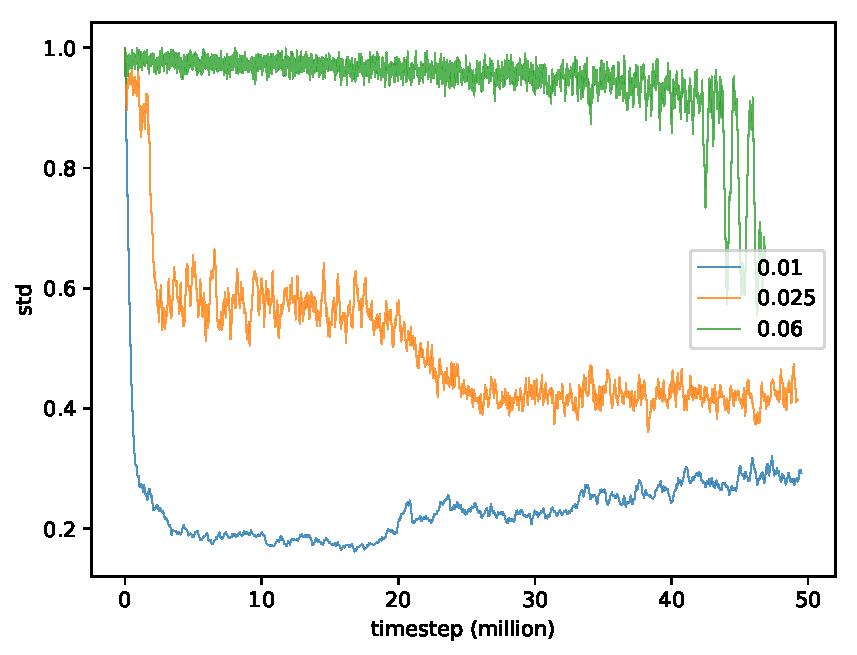
\includegraphics[width=\textwidth]{images/rec_180609_std_ent_reg.pdf}
	\centering
	\caption{Average standard deviation of the policy of agents in Figure~\ref{rec_ent_reg}, the horizontal axis is the number of million timesteps.}\label{rec_std_ent_reg}
\end{figure}

\subsection{Experiment on Exceptional Advantage Regularization}
The effectiveness of exceptional advantage regularization method on multi-modality tasks is discussed in this section.
First we demonstrate the general patterns of the distribution on the advantage values on the simple multi-modality task moveg2. The task samples a target direction from a set of 2 opposite directions at the beginning of each episode, and the agent is rewarded for moving toward the direction.

The experiment result on the average total reward of a normal ACKTR agent without any regularization is shown in Figure~\ref{rec_stat_moveg2}. The average reward per time-step during training is shown in Figure~\ref{rec_stat_moveg2_meanrt}, and the average standard deviation is shown in Figure~\ref{rec_stat_moveg2_std}.


\begin{figure}[!htbp]
	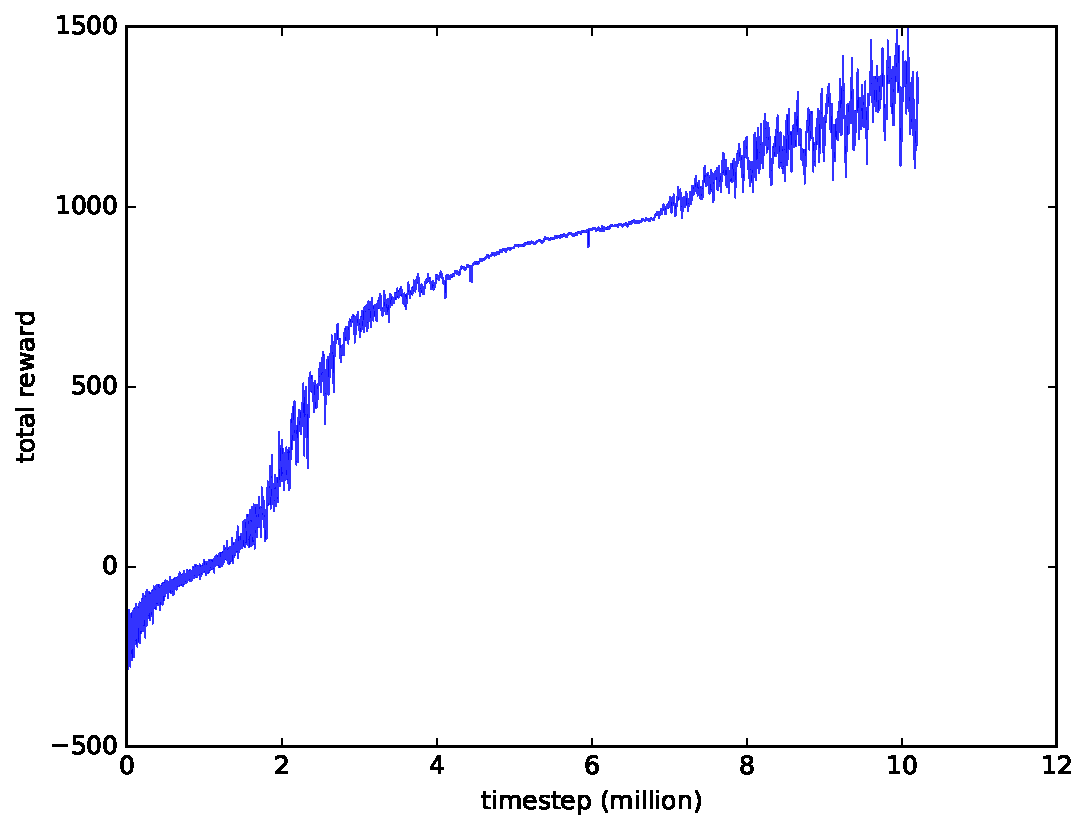
\includegraphics[width=0.7\textwidth]{images/rec_180528_statlog.pdf}
	\centering
	\caption{Performance of ACKTR agent on the moveg2 task, the horizontal axis is the number of million timesteps and the vertical axis is the total episode reward averaged over the last 20 episodes}\label{rec_stat_moveg2}
\end{figure}

\begin{figure}[!htbp]
	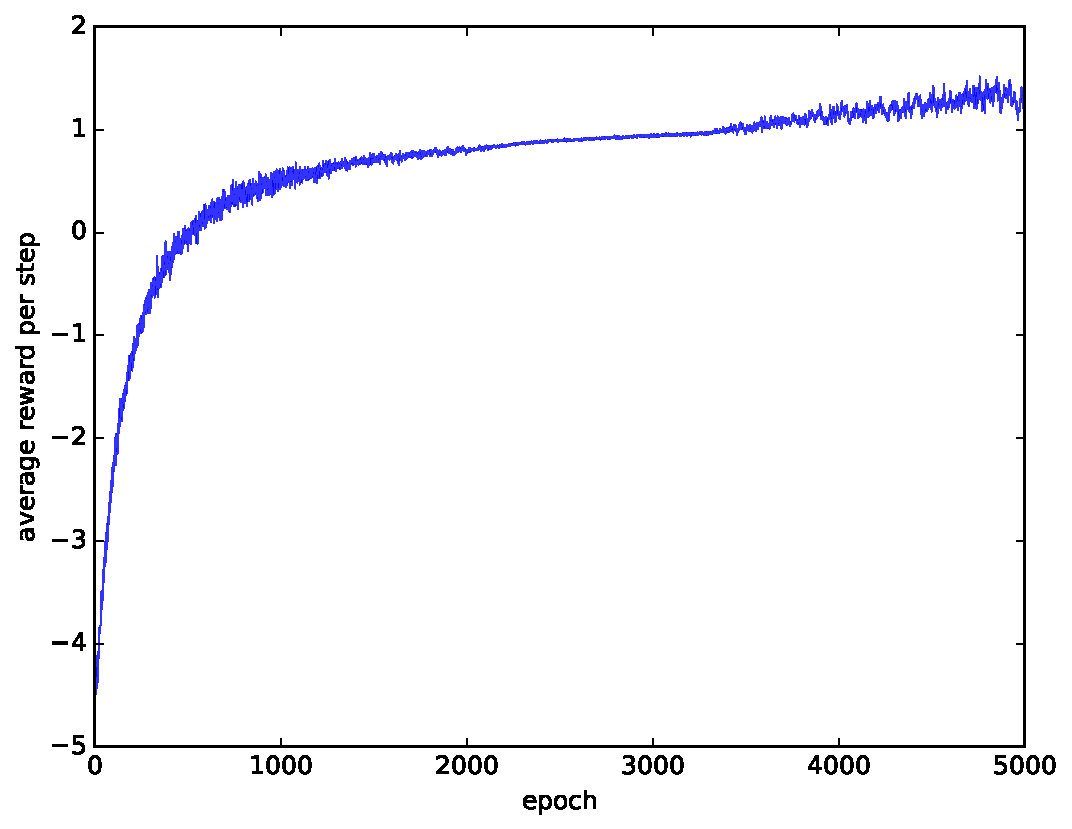
\includegraphics[width=0.7\textwidth]{images/rec_180528_meanrt_statlog.pdf}
	\centering
	\caption{The average reward per time-step of ACKTR agent on the moveg2 task, the horizontal axis is the number of training batches}\label{rec_stat_moveg2_meanrt}
\end{figure}

\begin{figure}[!htbp]
\label{key}	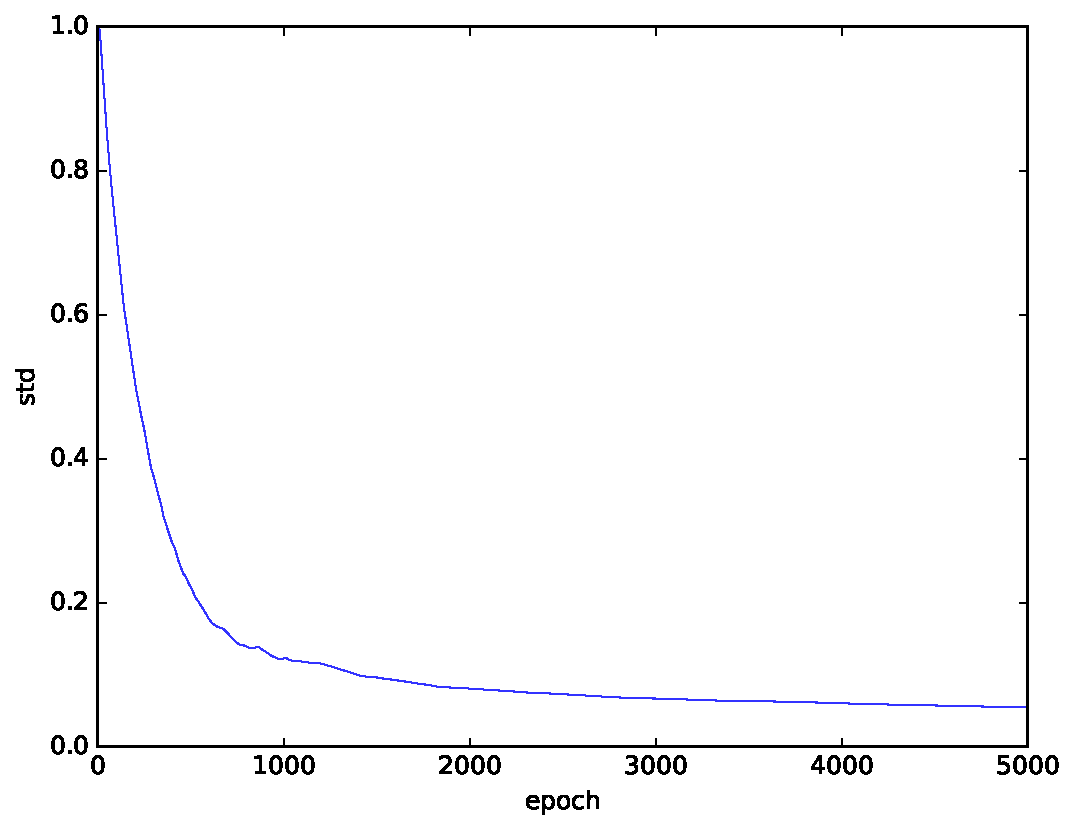
\includegraphics[width=0.7\textwidth]{images/rec_180528_std_statlog.pdf}
	\centering
	\caption{The average standard deviation of ACKTR agent's policy on the moveg2 task, the horizontal axis is the number of training batches}\label{rec_stat_moveg2_std}
\end{figure}
The distribution of advantage values at the first epoch (epoch 0) is shown in Figure~\ref{vis_stats_0}. It can be seen that the advantage values are distributed uniformly because the critic model is just initialized. Figure~\ref{vis_stats_3000} shows the distribution at epoch 3000. It can be seen that after the critic model has been trained for some time, the marginal distribution advantage value tend to follow a normal distribution with zero mean.  Figure~\ref{vis_stats_4900} shows the distribution of advantage values at epoch 4900. The advantage values are likely to have a positive bias at some samples with low log-likelihood  when the agent in this case, where the agent just managed to escape from a local minimum.  

A large number of samples with low likelihood but positive advantage value indicates that it might be beneficial to the agent if the degree of exploration is increased. However, figure~\ref{rec_stat_moveg2_std} on the change of average standard deviation shows that the agent actually keeps decreasing the standard deviations of its policy even at this case. Therefore, the application of an exceptional advantage regularization term, aims to solve this problem.
\begin{figure}[!htbp]
	\centering
	\begin{subfigure}[t]{0.5\textwidth}
		\centering
		\includegraphics[width=\textwidth]{vis_stats_0}
		\caption{Epoch 0}
			\label{vis_stats_0}
	\end{subfigure}%
	~ 
	\begin{subfigure}[t]{0.5\textwidth}
		\centering
		\includegraphics[width=\textwidth]{vis_stats_3000}
		\caption{Epoch 3000}
			\label{vis_stats_3000}
	\end{subfigure}
	~ 
	\begin{subfigure}[t]{0.7\textwidth}
		\centering
		\includegraphics[width=\textwidth]{vis_stats_4900}
		\caption{Epoch 4900}
		\label{vis_stats_4900}
	\end{subfigure}
	\caption{The distribution of advantage values of the ACKTR agent at epoch 0, 3000 and 4900 respectively. The horizontal axis is the log-likelihood value}
\end{figure}
%\begin{figure}[!htbp]
%	\includegraphics[width=\textwidth]{images/vis_stats_0.pdf}
%	\centering
%	\caption{The distribution of advantage values of the ACKTR agent at batch 0 on the moveg2 task, the horizontal axis is the log-likelihood value}
%	\label{vis_stats_0}
%\end{figure}
%
%\begin{figure}[!htbp]
%	\includegraphics[width=\textwidth]{images/vis_stats_3000.pdf}
%	\centering
%	\caption{The distribution of advantage values of the ACKTR agent at batch 300 on the moveg2 task, the horizontal axis is the log-likelihood value}
%	\label{vis_stats_3000}
%\end{figure}
%
%\begin{figure}[!htbp]
%	\includegraphics[width=\textwidth]{images/vis_stats_4900.pdf}
%	\centering
%	\caption{The distribution of advantage values of the ACKTR agent at batch 4900 on the moveg2 task, the horizontal axis is the log-likelihood value}
%	\label{vis_stats_4900}
%\end{figure}

The performance of exceptional advantage regularization (EAR) technique is tested on the 'movecont' task. We keep the same neural network configuration as in section \ref{sec_multi_modal_flat}, with the modification that the EAR technique is used.
The experiment result on the performance of an ACKTR agent with different weights exceptional advantage regularization is shown in Figure~\ref{rec_adv_reg}. The average standard deviation of the policies is also shown in Figure~\ref{rec_std_adv_reg}. All the agents are trained with batch-size 2560 and KL-divergence constraint 0.0003. The weight-0 agent is the same as the original ACKTR agent without any exploration regularization, and it could only achieve a total reward of around 2000 at the end of training. The agent with exceptional advantage regularization weight 0.04 can improve rapidly in the early phase before 40 million timestep, but gets stuck at around 3500. This shows that the exceptional advantage regularization method might cause an adverse effect on the final performance. The agent with exceptional advantage regularization weight 0.01 achieves the best final performance. Its average standard deviation shows that the agent manages to increase its policy entropy and re-explore the environment after it has escaped from a local minimum.
\begin{figure}[!htbp]
	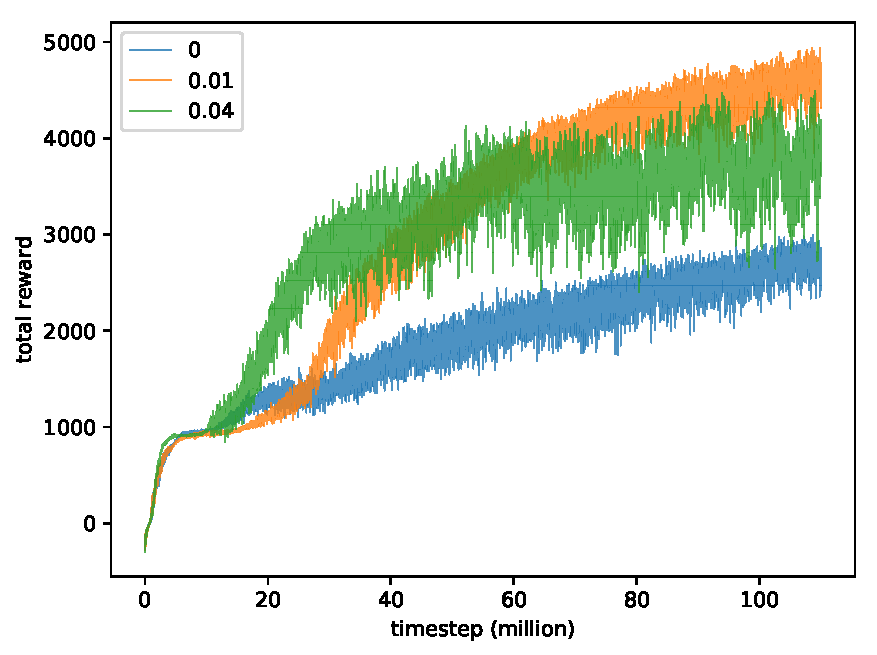
\includegraphics[width=\textwidth]{images/rec_180606_adv_reg.pdf}
	\centering
	\caption{Performance of agents with different exceptional advantage regularization weights, the horizontal axis is the number of million time-steps and the vertical axis is the total episode reward averaged over the last 32 episodes}\label{rec_adv_reg}
\end{figure}

\begin{figure}[!htbp]
	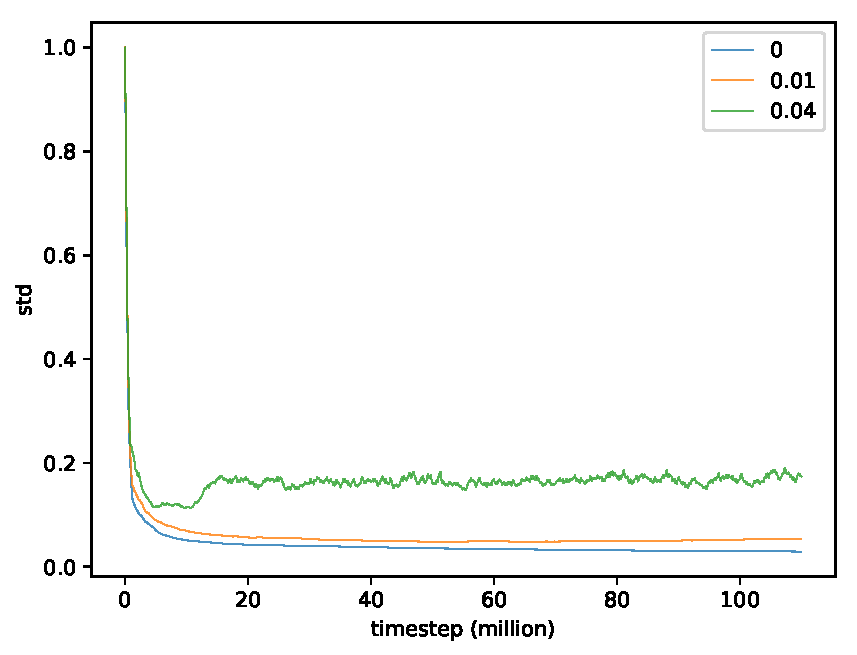
\includegraphics[width=\textwidth]{images/rec_180606_std_adv_reg.pdf}
	\centering
	\caption{The average standard deviation of agents with different exceptional advantage regularization weights, the horizontal axis is the number of million time-steps and the vertical axis is the total episode reward averaged over the last 32 episodes}\label{rec_std_adv_reg}
\end{figure}

\subsection{Experiment on Robust Concentric Gaussian Mixture Policy Model}
The effectiveness of robust concentric Gaussian mixture policy agent in exploration of task movecont is tested in this section. We use the same configuration as in section \ref{sec_multi_modal_flat} except that the distribution type is changed to the robust concentric Gaussian mixture policy. We use the empirical estimation of the KL-divergence since there is no closed-form solution on it.

The experiment result on the performance of an ACKTR Gaussian mixture policy agent is shown in Figure~\ref{rec_mix}. The Gaussian mixture policy agents have slower rates on performance improvement compared to pure Gaussian policy agents. However, the agent is still able to achieve a good final performance, with a total reward of around 4000.

\begin{figure}[!htbp]
	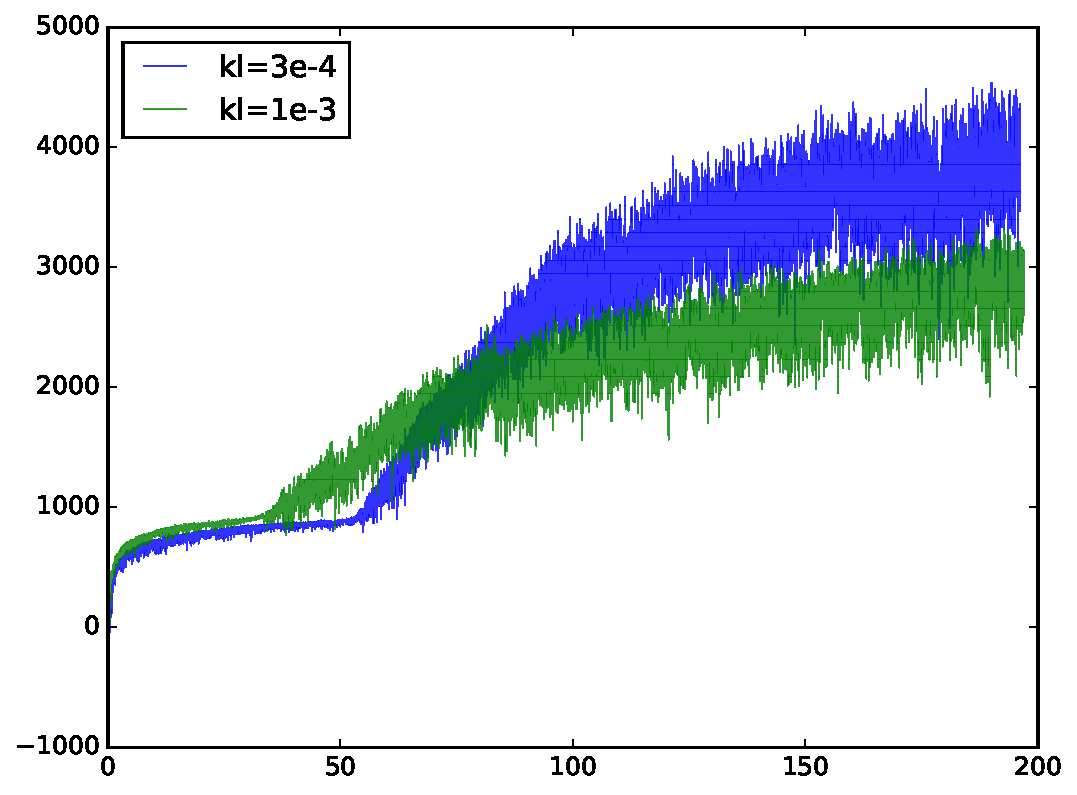
\includegraphics[width=\textwidth]{images/rec_180612_mix.pdf}
	\centering
	\caption{Performance of ACKTR agents with different KL-divergence constraints, the horizontal axis is the number of million time-steps and the vertical axis is the total episode reward averaged over the last 32 episodes.}\label{rec_mix}
\end{figure}
